\chapter{Chapter}
Chapters are in chapters folder. Each chapter is a separate file. All chapters must be referenced in the thesis.tex file. Document should be built pointing the thesis.tex file. Other files do not have document beginning.
\section{Section}
This is a section. A title in your chapter. Sections can be further devided in to sub-sections and subsub-sections.

Originally, Balrogs were Maiar that were later persuaded by Melkor before the Awakening of the Elves. Their first dwellings had been Utumno, but after their master's defeat during the War for Sake of the Elves, the Balrogs and other creatures in Melkor's service escaped and went to Angband\footnote{http://lotr.wikia.com/wiki/Angband}.
\subsection{Sub Section}
	This is a subsection and they get listed in the TOC(Table Of Content).
\subsubsection{Sub Sub Section}
	This is a sub sub section and they do not get listed on TOC.	
\section{Figures}
Figures should  be referenced before the actual figure in the text. Figure \ref{bounding} depicts the left side view of the death star. 
	\begin{figure}[H]
		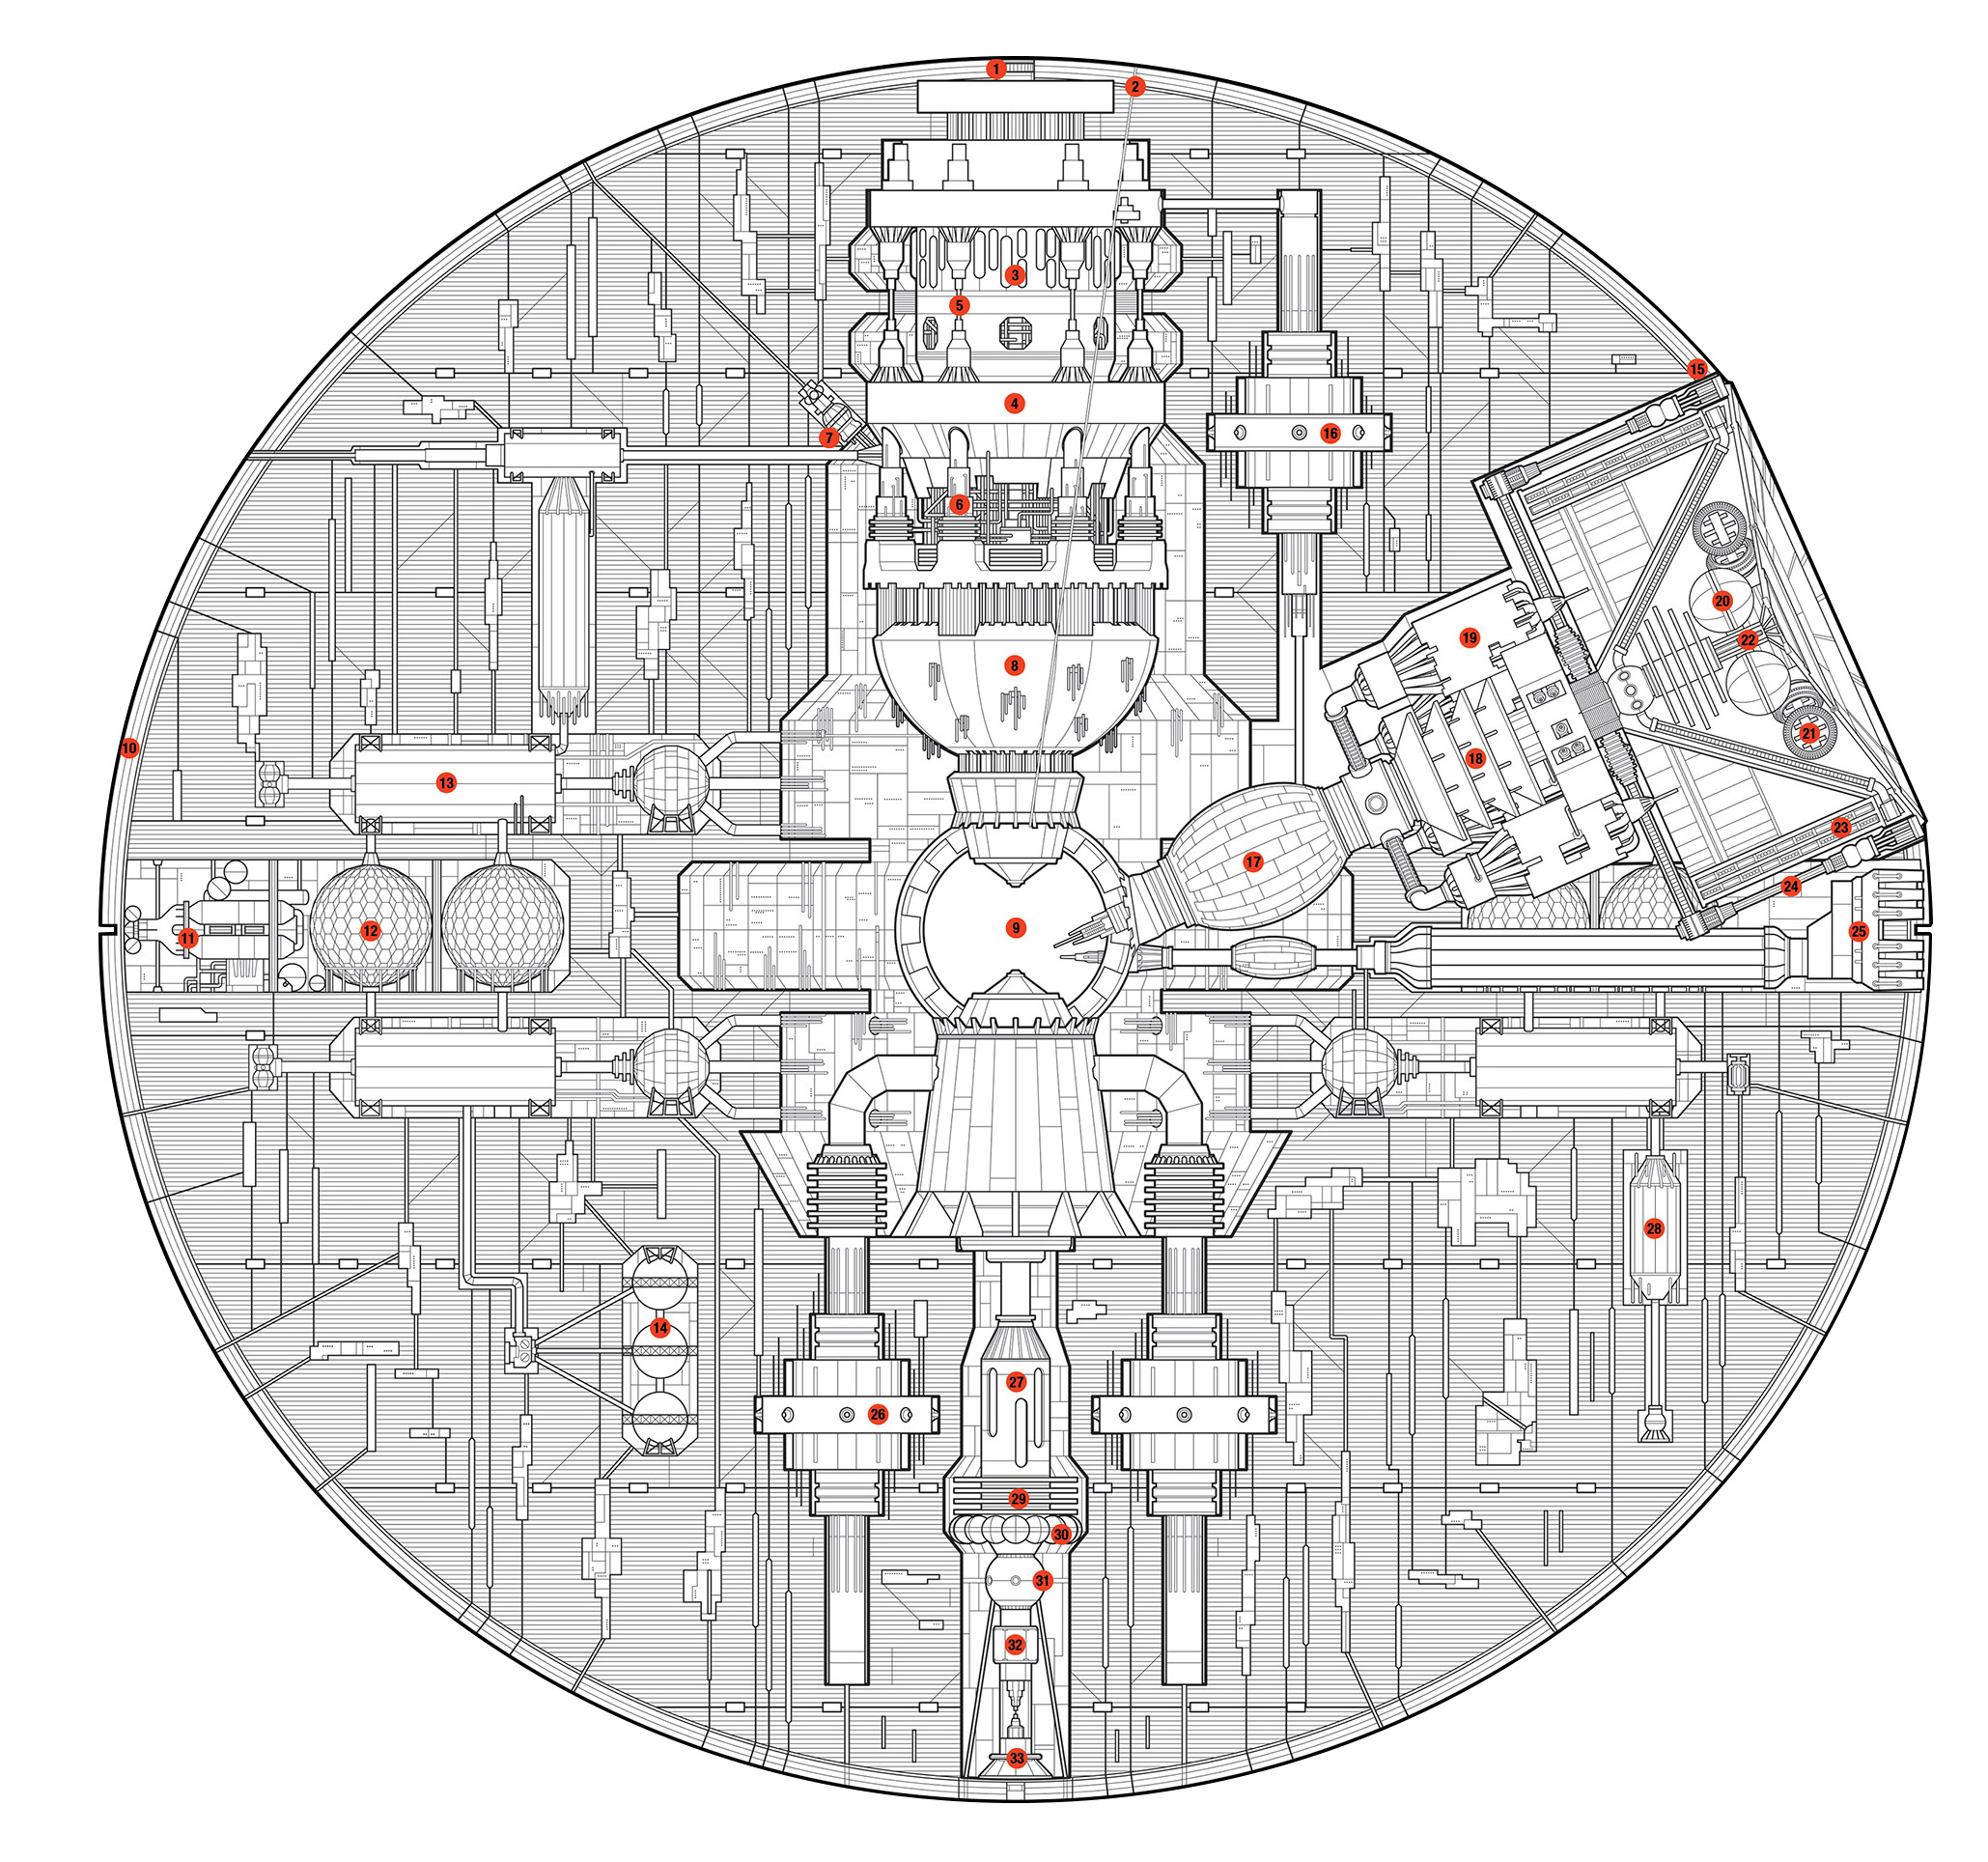
\includegraphics[width=8cm]{a.jpg}
		\centering
		\caption{Death star, left side view}
		\label{bounding}
	\end{figure}

\section{Un-ordered List}
	
\begin{itemize}
	\item Item 1
	\item Item 2
	\item Item 3
	\item Item 4
	\item Item 5
\end{itemize}

\section{Ordered List}

\begin{enumerate}
	\item One item
	\item Another item
	\item And another one
\end{enumerate}

\section{Table}
Tables should be referenced in the text before the appearance of the table. Table \ref{acc_cross} shows some numbers and by decoding it you prove that the answer for life and everything is 42.
\begin{table}[H]
\centering
\caption{Some numbers with titles}
\label{acc_cross}
\vspace{0.4cm}
\begin{tabular}{|l|l|l|l|l|l|}
\hline
\# & Epochs & LR      & Batch size & LSB  & RSB  \\ \hline
1.1  & 50     & 0.1     & 10         & NA   & NA   \\ \hline
1.2  & 50     & 0.01    & 10         & 36\% & 31\% \\ \hline
1.3  & 50     & 0.001   & 10         & 41\% & 36\% \\ \hline
1.4  & 50     & 0.0001  & 10         & 43\% & 37\% \\ \hline
1.5  & 50     & 0.00001 & 10         & 40\% & 37\% \\ \hline
1.6  & 100    & 0.01    & 10         & 38\% & 31\% \\ \hline
\end{tabular}
\end{table}

\section{Bibliography}
Harvard ref style is used here. You can change the style as you prefer. \citep{ban2014} or \citet{ban2014}.